\chapter{Результаты проектирования системы ролевой игры с виртуальным мастером}

В данной главе описывается архитектура разработанной системы ролевой игры с виртуальным мастером. Представлено детальное описание основных подсистем, их интерфейсов и взаимодействия между компонентами.


\section{Общая архитектура системы}

Разработанная система ролевой игры с виртуальным мастером построена на основе объектно-ориентированной архитектуры с использованием асинхронного программирования. Система организована в виде модульной структуры, где каждый компонент отвечает за определённую функциональность.

Основные компоненты системы и их взаимодействие представлены на рис.~\ref{fig:system-architecture}.
\begin{figure}[ht]
	\centering
	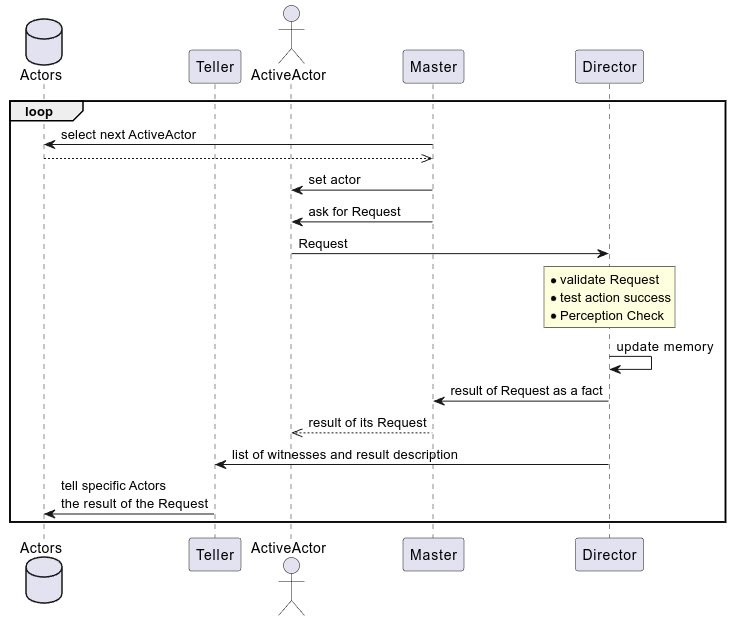
\includegraphics[width=0.8\linewidth]{img/pic1.jpg}
	\caption{Общая архитектура системы ролевой игры с виртуальным мастером}
	\label{fig:system-architecture}
\end{figure}

Класс \texttt{Game} является точкой входа в систему и управляет основным игровым циклом. Он координирует работу компонентов \texttt{Plot}, содержащего последовательность сцен, и \texttt{Storyteller}, генерирующего повествование.

Каждая сцена (\texttt{Scene}) содержит набор персонажей и компоненты для управления взаимодействием: \texttt{Director} для выдачи директив, \texttt{SceneJudge} для проверки корректности действий, \texttt{SceneChanger} для определения завершения сцены.

Неигровые персонажи (\texttt{MCharacter}) управляются через класс \texttt{Agent}, который использует \texttt{Brain} для моделирования эмоционального состояния и \texttt{Interface} для взаимодействия с большими языковыми моделями.

Компонент \texttt{Dice} обеспечивает разрешение механических проверок действий, используя \texttt{Interface} для определения необходимости проверки и её параметров.


\section{Архитектура подсистемы управления игровым циклом}

Подсистема управления игровым циклом реализована в классе \texttt{Game}. Основные методы класса:

\begin{itemize}
	\item \texttt{\_\_init\_\_(plot, player, storyteller)} --- инициализация игры с заданным сюжетом, персонажем игрока и генератором повествования.
	
	\item \texttt{runGame()} --- основной асинхронный метод, реализующий игровой цикл. Метод последовательно обрабатывает сцены, координируя работу компонентов генерации повествования, выдачи директив и обработки действий.
	
	\item \texttt{\_get\_current\_scene()} --- получение текущей активной сцены из сюжета.
\end{itemize}

Класс \texttt{Game} хранит состояние текущей сцены (\texttt{current\_scene\_index}) и текущего действия (\texttt{current\_action}), что позволяет корректно обрабатывать переходы между сценами.

\section{Архитектура подсистемы управления сценами}

Подсистема управления сценами реализована в классе \texttt{Scene}. Сцена содержит следующие компоненты:

\begin{itemize}
	\item \texttt{director} --- компонент выдачи директив неигровым персонажам.
	
	\item \texttt{scene\_judge} --- компонент проверки корректности действий персонажей.
	
	\item \texttt{scene\_changer} --- компонент определения завершения сцены.
	
	\item \texttt{master\_characters} --- список неигровых персонажей в сцене.
	
	\item \texttt{player} --- персонаж игрока.
\end{itemize}

Основной метод \texttt{give\_spotlight(spotlight)} обрабатывает выдачу директивы персонажу:

\begin{enumerate}
	\item Определение типа персонажа (игрок или неигровой персонаж).
	
	\item Для игрока: запрос действия через консольный ввод с валидацией через \texttt{PCharacter.judge()}.
	
	\item Для неигрового персонажа: генерация ответа через \texttt{MCharacter.get\_replic\_to()}.
	
	\item Проверка корректности действия через \texttt{SceneJudge.judge()}.
	
	\item Разрешение действия через \texttt{Dice.resolve\_action()} при необходимости.
	
	\item Определение персонажей, воспринявших действие, через \texttt{SceneJudge.perception\_check()}.
	
	\item Обновление памяти всех воспринявших действие персонажей.
\end{enumerate}

\section{Архитектура подсистемы выдачи директив}

Подсистема выдачи директив реализована в классе \texttt{Director}. Компонент анализирует текущее состояние игры и выдаёт директивы неигровым персонажам для продвижения сюжета.

Класс \texttt{Director} содержит:
\begin{itemize}
	\item \texttt{plot} --- описание сюжета текущей сцены.
	
	\item \texttt{ai} --- интерфейс для взаимодействия с большими языковыми моделями.
	
	\item \texttt{messages} --- история сообщений, используемая для контекста при генерации директив.
\end{itemize}

Метод \texttt{give\_directive(story\_information)} формирует директиву следующим образом:

\begin{enumerate}
	\item Добавление текущей информации о ситуации в историю сообщений.
	
	\item Формирование промпта, описывающего роль мастера игры и текущую ситуацию.
	
	\item Генерация директивы через \texttt{Interface.extract\_text()}.
	
	\item Парсинг ответа для извлечения имени персонажа и содержания директивы.
	
	\item Возврат объекта \texttt{Spotlight}.
\end{enumerate}

\section{Архитектура подсистемы управления персонажами}

Подсистема управления персонажами включает классы \texttt{Character}, \texttt{MCharacter}, \texttt{PCharacter} и \texttt{Agent}.

Базовый класс \texttt{Character} содержит общие атрибуты:
\begin{itemize}
	\item \texttt{name} --- имя персонажа.
	
	\item \texttt{stats} --- объект класса \texttt{Stats}, содержащий характеристики персонажа (сила, ловкость, выносливость, интеллект, мудрость, харизма).
	
	\item \texttt{background} --- предыстория персонажа.
	
	\item \texttt{aspects} --- список аспектов персонажа.
\end{itemize}

Класс \texttt{MCharacter} расширяет \texttt{Character} и добавляет:
\begin{itemize}
	\item \texttt{agent} --- объект класса \texttt{Agent}, управляющий поведением персонажа.
	
	\item Метод \texttt{get\_replic\_to(instruction)} --- генерация ответа на директиву через агента.
	
	\item Метод \texttt{erase\_last\_memory()} --- удаление последнего сообщения из памяти агента.
	
	\item Метод \texttt{update\_memory(memory)} --- обновление памяти агента новыми событиями.
\end{itemize}

Класс \texttt{PCharacter} представляет персонажа игрока и содержит:
\begin{itemize}
	\item \texttt{ai} --- интерфейс для проверки корректности действий игрока.
	
	\item Метод \texttt{judge(request, history)} --- проверка соответствия действия предыстории персонажа и логике игры.
\end{itemize}

\section{Архитектура подсистемы эмоционального моделирования}

Подсистема эмоционального моделирования реализована в классах \texttt{Brain} и \texttt{MoralScheme}.

Класс \texttt{MoralScheme} инкапсулирует моральную схему персонажа:
\begin{itemize}
	\item \texttt{base\_intentions} --- словарь базовых намерений персонажа.
	
	\item \texttt{appraisals} --- вектор оценок текущей ситуации.
	
	\item \texttt{feelings} --- вектор эмоционального состояния.
	
	\item Методы \texttt{update\_vectors(action)} --- обновление векторов на основе нового действия.
	
	\item Метод \texttt{euc\_dist()} --- вычисление расстояния между оценками и чувствами.
\end{itemize}

Класс \texttt{Brain} управляет одной или несколькими моральными схемами:
\begin{itemize}
	\item Поддержка одиночной схемы (\texttt{multi = False}) или множественных схем (\texttt{multi = True}).
	
	\item Метод \texttt{current()} --- получение текущей активной схемы.
	
	\item Метод \texttt{switch\_to(scheme\_idx)} --- переключение между схемами.
	
	\item Метод \texttt{check\_transition(scheme\_idx, context)} --- проверка условий перехода между схемами.
\end{itemize}

Класс \texttt{Agent} использует \texttt{Brain} для управления поведением персонажа:
\begin{itemize}
	\item Метод \texttt{analyze\_intentions(user\_text)} --- анализ намерений во входном тексте.
	
	\item Метод \texttt{analyze\_emotions(user\_text)} --- анализ эмоций во входном тексте.
	
	\item Метод \texttt{generate\_reply(user\_text)} --- генерация ответа с учётом эмоционального состояния.
\end{itemize}

\section{Архитектура подсистемы взаимодействия с большими языковыми моделями}

Подсистема взаимодействия с большими языковыми моделями реализована в классе \texttt{Interface}. Компонент обеспечивает абстракцию над HTTP API больших языковых моделей.

Основные методы класса:
\begin{itemize}
	\item \texttt{post\_messages(messages, model)} --- отправка сообщений в API и получение JSON-ответа.
	
	\item \texttt{extract\_text(messages, model)} --- извлечение текстового содержимого из ответа API.
	
	\item \texttt{get\_composition(intents, phrase, model)} --- получение вектора вероятностей намерений для заданной фразы.
\end{itemize}

Класс поддерживает конфигурирование через файл \texttt{config.yaml}, позволяя задавать:
\begin{itemize}
	\item Провайдера API (OpenAI, прокси и т.д.).
	
	\item API ключ и базовый URL.
	
	\item Модель для использования (по умолчанию \texttt{gpt-4o-mini}).
\end{itemize}


\section{Выводы}

В результате проектирования системы ролевой игры с виртуальным мастером получены следующие инженерные результаты:

\begin{enumerate}
	\item Спроектирована модульная архитектура системы, организованная в виде иерархии подсистем: управления игровым циклом, управления сценами, выдачи директив, управления персонажами, эмоционального моделирования, разрешения действий и взаимодействия с большими языковыми моделями.
	
	\item Разработаны интерфейсы взаимодействия между компонентами системы, обеспечивающие слабую связанность и возможность независимого развития подсистем. Все взаимодействия реализованы через асинхронные методы, что обеспечивает возможность параллельной обработки запросов.
	
	\item Интегрирована система управления эмоциональным состоянием персонажей на основе моральных схем, обеспечивающая динамическое изменение поведения персонажей в зависимости от их взаимодействий. Система поддерживает как одиночные, так и множественные моральные схемы с возможностью переключения между ними.
	
	\item Разработана архитектура компонента выдачи директив, который анализирует текущее состояние игры и выдаёт директивы неигровым персонажам для продвижения сюжета, обеспечивая баланс между свободой действий игрока и следованием задуманному сюжету.
	
	\item Спроектирована система разрешения действий, интегрирующая механические элементы игры (броски кубиков, проверки характеристик) с генерацией повествования. Система использует большие языковые модели для определения необходимости проверок и их параметров, обеспечивая согласованность между механическими правилами и описанием происходящего.
\end{enumerate}

Отличительной особенностью разработанной архитектуры является интеграция структурированного управления состоянием игры с генеративными возможностями больших языковых моделей, что обеспечивает более контролируемый и согласованный игровой процесс по сравнению с чисто генеративными решениями.

%%% Local Variables:
%%% TeX-engine: xetex
%%% eval: (setq-local TeX-master (concat "../" (seq-find (-cut string-match ".*-3-pz\.tex$" <>) (directory-files ".."))))
%%% End:
